\itemhead{习题3.1 · 第10题（教材p.77）}{XJ-B1-C03-HW-P077-Y1356}
\label{XJ-B1-C03-HW-P077-Y1356}
{\footnotesize 湘教版教材p.77 / PDF第84页 / 习题3.1 / 第10题}
\field{原题}{滑雪运动员以恒定加速度沿着笔直的雪道向下滑。在 $t=0$ 时刻，他以 $6\,\mathrm{m/s}$ 的速度经过点 $A$，然后加速下滑直到以 $15\,\mathrm{m/s}$ 的速度经过点 $B$。在 $B$ 点，雪道开始变平，他从 $B$ 点开始以恒定速度 $15\,\mathrm{m/s}$ 滑到 $C$ 点。已知 $A,C$ 之间的路程是 $615\,\mathrm m$，他从 $B$ 点滑到 $C$ 点用了 $20\,\mathrm s$。
\subq{1}求出 $A,B$ 之间的路程；
\subq{2}求该运动员从 $A$ 滑到 $B$ 的时间；
\subq{3}画出该运动员滑雪的速度-时间图象。}
\field{参考答案}{（1）$AB=615-15\times20=315$ m；（2）$t_{AB}=315/[(6+15)/2]=30$ s；（3）图象为 $(0,6)$ 到 $(30,15)$ 的线段，再连接 $(50,15)$。即 $v=6+0.3t$（$0\le t\le30$）、$v=15$（$30<t\le50$）。}
\begin{center}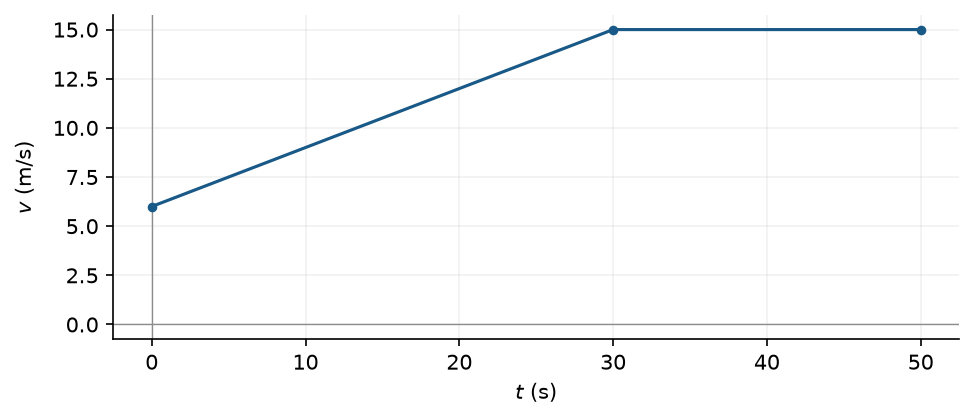
\includegraphics[width=.84\linewidth,height=.38\textheight,keepaspectratio]{figures/C03-HW077-10.png}\end{center}
{\small \field{关联知识}{F07 分段函数、绝对值及分段应用（教材帮p.86、91、92、93 / PDF95、100、101、102）；F04 函数三种表示法、图象与读数（教材帮p.85、86、93、94 / PDF94、95、102、103）}
\field{方法与易错点}{先列转折点和各段条件，再建立分段式，检查衔接、定义域与值域。 易错：跨段套公式；超额部分按全量收费；绝对值去号漏区间。}
\field{答案依据}{答案册相关题组：PDF第20、21、22页（册内页19、20、21）；按当前题库原题逐项重算，不按旧版题号机械对套。}}
